\subsection{Real data}\label{res_real_data}

In this section, the results that will be presented are obtained on real data.
The main dataset that we will be using is called \textit{sample}, as it simply is the sample data available on the \texttt{MNE} package.
In this experiment, checkerboard patterns were presented to the subject into the left and right visual field, interspersed by tones to the left or right ear.
The interval between the stimuli was 750 ms.
Occasionally a smiley face was presented at the centre of the visual field.
The subject was asked to press a key with the right index finger as soon as possible after the appearance of the face\footnote{Source: \href{https://mne.tools/0.11/manual/datasets_index.html}{MNE documentation}}.
In the following, we are only interested in the four main stimuli types: auditory left, auditory right, visual left and visual right.
The experiment lasts about \SI{4.6}{\minute} and approximately 70 stimuli per type was presented, with a minimum of \SI{2.5}{\second} between two stimuli  of the same type.

As previously explained, the recorded signals must first of all be decomposed in $K$ atoms.
In our case, we put $K=40$, and some examples of obtained atoms were presented in Figure~\ref{fig:atom_location_and_form}.

Unlike the previous section where the data were simulated and thus the real values of the parameters were known, now we do not have any ground truth to compare our results to.
Thus, we will focus on showing that the algorithm converges on real data too.
However, with some domain expertise, one is able to determine the origin of a given atom.
For example, the atom 0 in Figure~\ref{fig:atom_location_and_form}, the one on the left, is characteristic of an heartbeat, which is confirmed by its spatial pattern which represents a diffuse area rather than a specific zone, as the heartbeat comes from \say{under} the brain, approximately form the middle left.
Similarly, the atom 1, the one in the middle, can easily be associated with the subject's eye blinks.
Thus, even if we do not have a ground truth, as we do not know which atom is linked to which stimulus, it can be said that some specific atoms are not linked to any stimulus, as it is the case with the heartbeat atom, for which it is reasonable to say that it is not influenced by any stimulus.
Note that such a statement is not as clear for the eye blinks atom, as the subject can eventually anticipate the incoming visual stimuli and therefore make an effort to not blink accordingly.

Let us first fit a model for atom 2, the one on the right in Figure~\ref{fig:atom_location_and_form}, alongside tasks 1 and 2, respectively the auditory on the left side stimulus and  the auditory on the right side stimulus.
We combine those two stimuli using the method presented in Equation~\eqref{eq:intensity_combined_stimuli}.
Combining those two stimuli make sens as it is understandable that two auditory stimuli would generate a similar activation in the brain.
This is confirmed by the atom's spatial representation, which has a certain axial symmetry.
Loss and parameters convergence are shown in Figures~\ref{fig:history_loss_atom_2_task_1_2} and~\ref{fig:history_params_atom_2_task_1_2}.

\begin{figure}[h!]
    \centering
    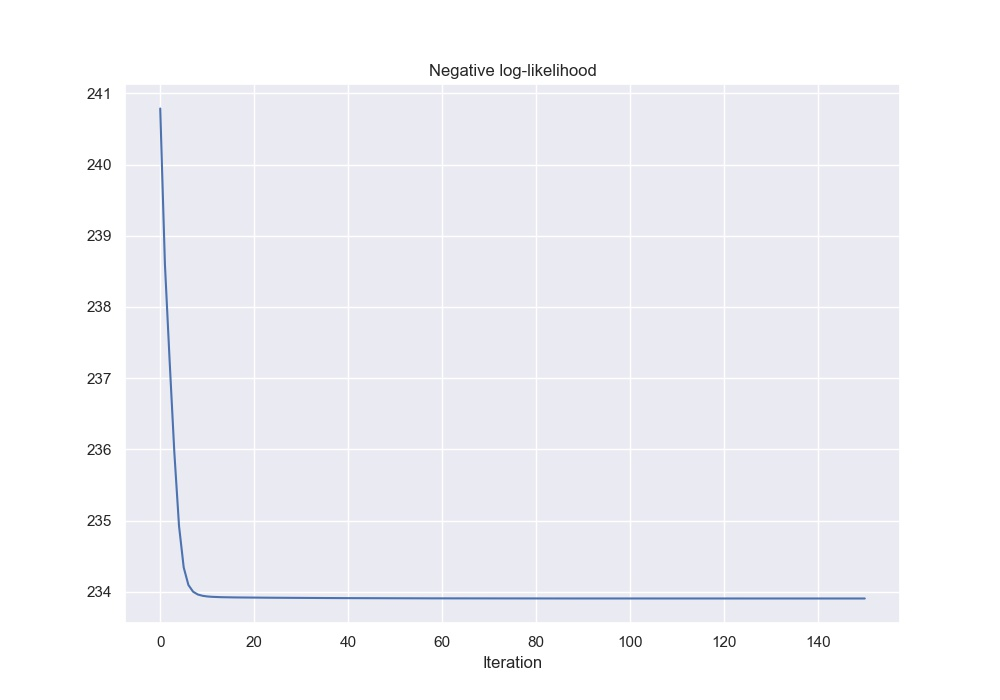
\includegraphics[width=0.9\textwidth]{pics/results_sample/history_loss_atom_2_task_1_2.jpg}
    \caption{Loss history over 150 iterations with a \textit{smart} initialisation, on sample data (atom 2, task 1 and 2) with $\intervalleFF{a}{b} = \intervalleFF{30}{800}\times \SI{e-3}{\second}$.}
    \label{fig:history_loss_atom_2_task_1_2}
\end{figure}

\begin{figure}[h!]
    \centering
    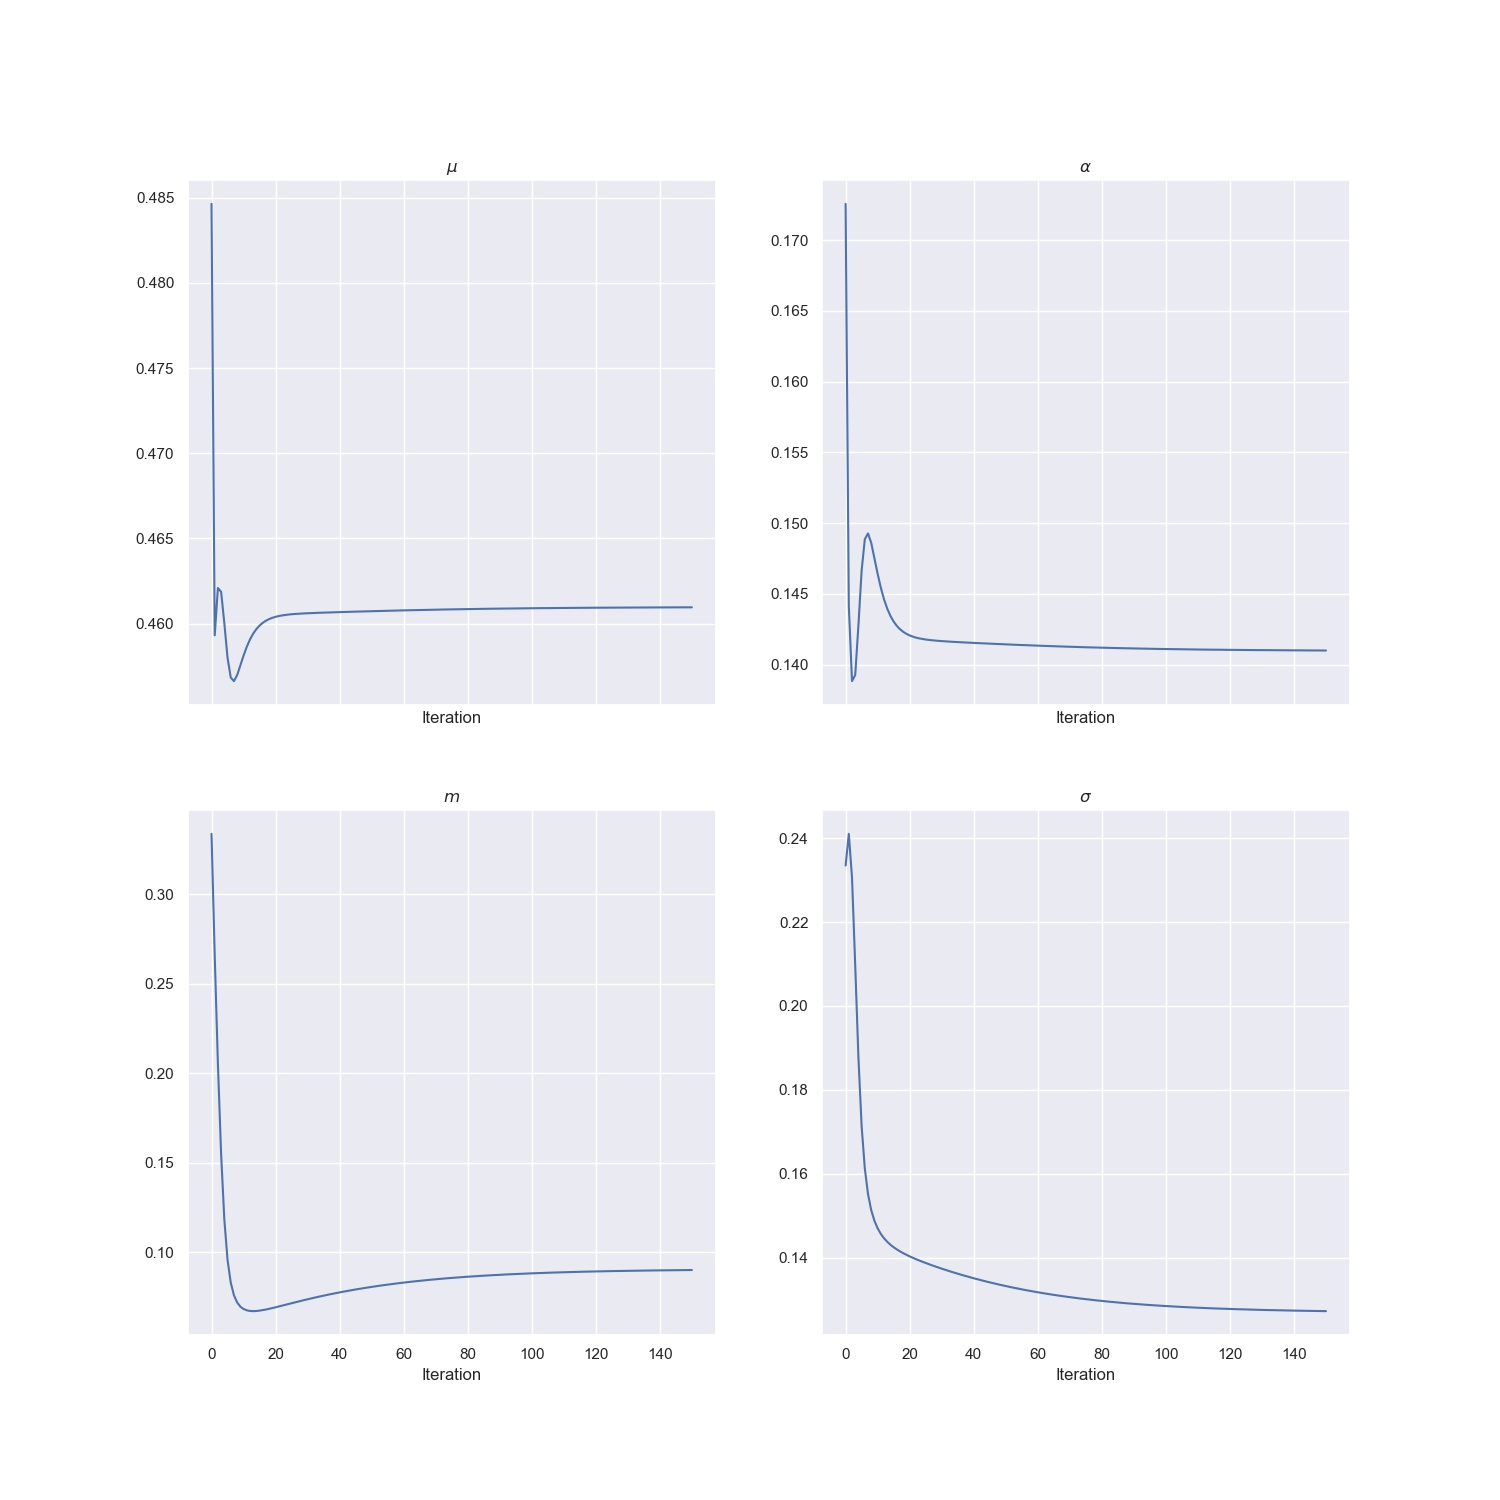
\includegraphics[width=\textwidth]{pics/results_sample/history_params_atom_2_task_1_2.jpg}
    \caption{Parameters recovery over 150 iterations with a \textit{smart} initialisation, on sample data (atom 2, task 1 and 2) with $\intervalleFF{a}{b} = \intervalleFF{30}{800}\times \SI{e-3}{\second}$.}
    \label{fig:history_params_atom_2_task_1_2}
\end{figure}

A similar experiment can be carried out on atom 0, the one that can be easily associated with a heartbeat, again alongside stimuli 1 and 2.
Loss and parameters convergence are shown in Figures~\ref{fig:history_loss_atom_0_task_1_2} and~\ref{fig:history_params_atom_0_task_1_2}.
When carried out alongside stimuli 3 and 4, respectively the visual left stimulus and the visual right stimulus, the initial value of $\alpha$ is null, thus no history is available as only the maximum likelihood estimator for the baseline parameter is computed, as mentioned in Section~\ref{parameters_initialisation}.
However, as there is no particular to consider atom 0 only alongside the auditory stimuli, one final experiment is carried out, this time by taking all of the stimuli.
Loss and parameters convergence are shown in Appendix~\ref{annexe:extra_results_real}, Figures~\ref{fig:history_loss_atom_0_task_1_2_3_4} and~\ref{fig:history_params_atom_0_task_1_2_3_4} respectively.

\begin{figure}[h!]
    \centering
    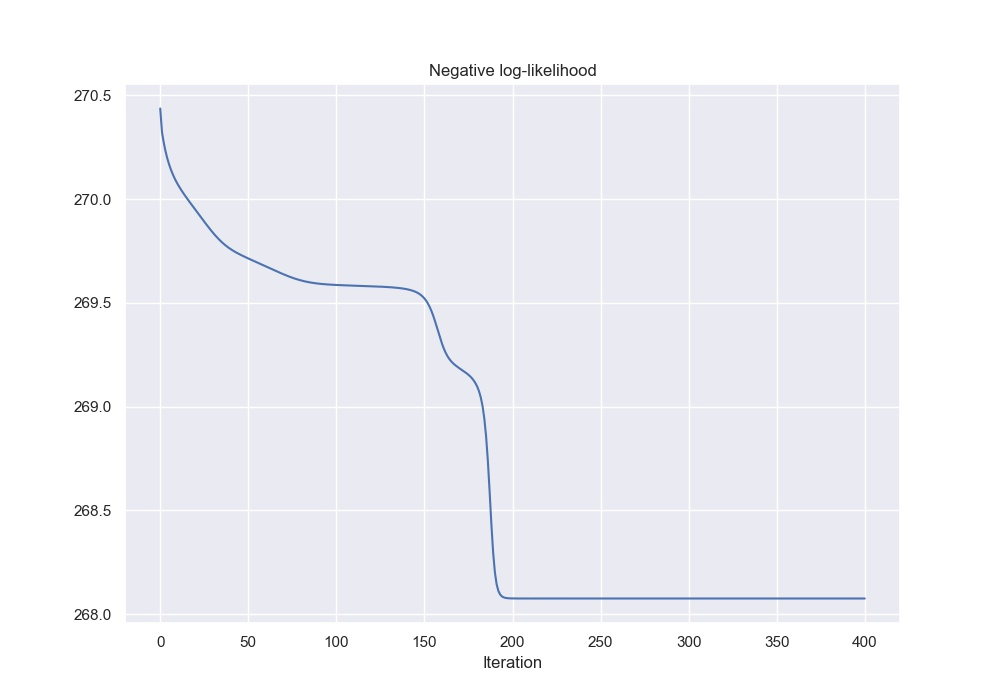
\includegraphics[width=0.9\textwidth]{pics/results_sample/history_loss_atom_0_task_1_2.jpg}
    \caption{Loss history over 400 iterations with a \textit{smart} initialisation, on sample data (atom 0, task 1 and 2) with $\intervalleFF{a}{b} = \intervalleFF{30}{800}\times \SI{e-3}{\second}$.}
    \label{fig:history_loss_atom_0_task_1_2}
\end{figure}

\begin{figure}[h!]
    \centering
    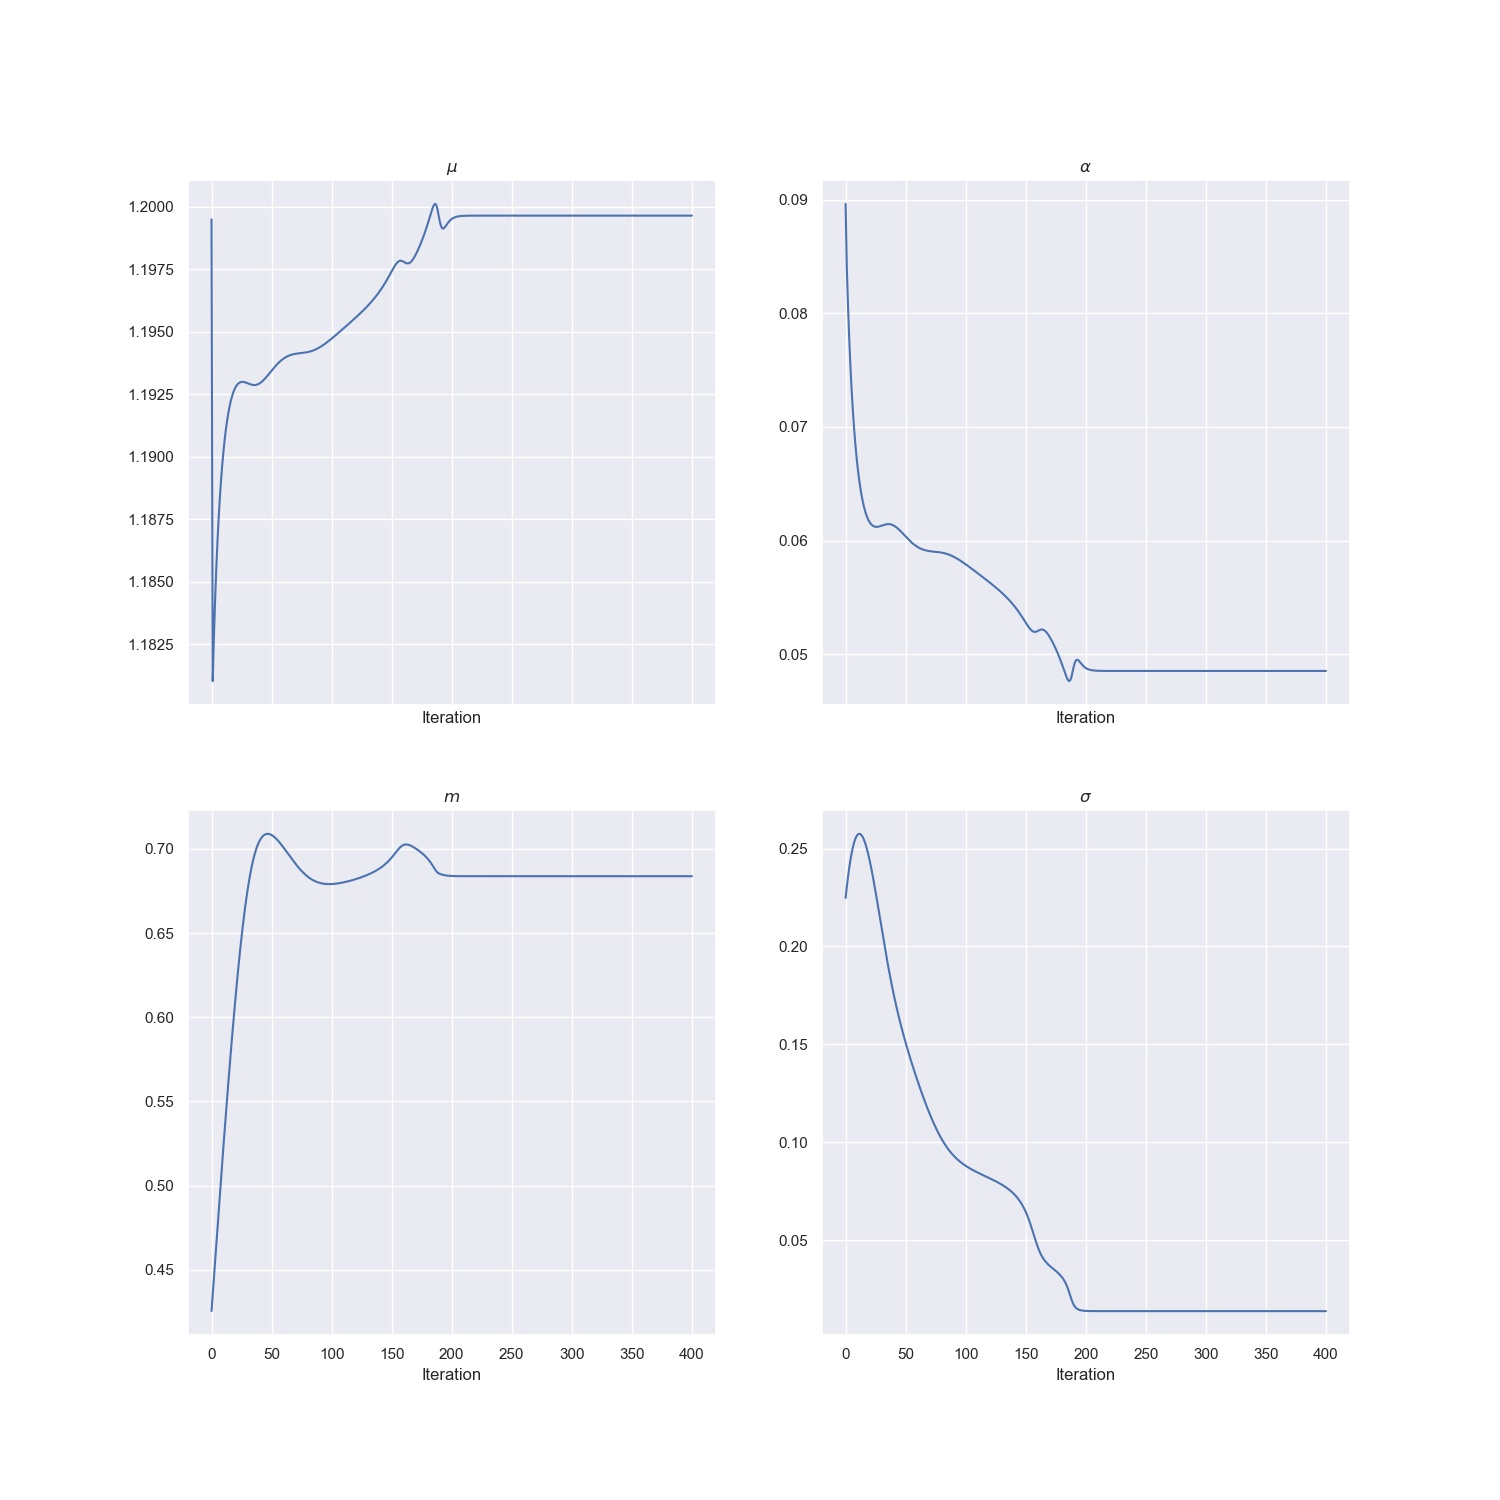
\includegraphics[width=\textwidth]{pics/results_sample/history_params_atom_0_task_1_2.jpg}
    \caption{Parameters recovery over 400 iterations with a \textit{smart} initialisation, on sample data (atom 0, task 1 and 2) with $\intervalleFF{a}{b} = \intervalleFF{30}{800}\times \SI{e-3}{\second}$.}
    \label{fig:history_params_atom_0_task_1_2}
\end{figure}

% TODO: Dire que si on connaît déjà le lien possible, on peut interpréter les résultats, parler de la mesure ration p\_a/p\_s. exemple sur sample de l'atoms lié aux battements de coeurs, qui par définition, ne doit pas avoir de lien avec aucun des task


